\chapter{Fat Pointer Based Range Addresses}

\ifpdf
    \graphicspath{{Fat-Pointer-Based-Range-Address/Figs/Raster/}{Fat-Pointer-Based-Range-Address/Figs/PDF/}{Fat-Pointer-Based-Range-Address/Figs/}}
\else
    \graphicspath{{Fat-Pointer-Based-Range-Address/Figs/Vector/}{Fat-Pointer-Based-Range-Address/Figs/}}
\fi


FAT-Pointers based range addresses, combined with the capabilities of the CHERI (Capability Hardware Enhanced RISC Instructions) 
architecture, introduce robust memory safety and security features by incorporating additional metadata 
with memory pointers. This enhanced architecture utilizes concepts such as FlexPointer, 
Range Memory Mapping (RMM) to manage memory effectively.

Range addresses play a pivotal role within this framework, defining memory 
regions bounded by a starting address (Upper) and an ending address (Lower). 
These range addresses are encoded within FAT-pointers, allowing for precise 
control over memory regions.

The functionality of ranges encompasses several key aspects:
\begin{itemize}
\item \textbf{Creation of Physically Contiguous Memory Ranges}:
By defining memory regions that are physically contiguous, systems can 
achieve optimal memory access patterns, enhancing performance and efficiency.
\item \textbf{Encoding Ranges as Bounds to the Pointer}:
Integrating range bounds directly into FAT-pointers enables the architecture 
to enforce memory access restrictions at the pointer level thus allowing 
tracking of memory ranges on a pointer level.
\item \textbf{Instrumenting Block-Based Allocators with Physically Contiguous Memory}:
The integration of range-based memory concepts into memory allocation systems, such as block-based 
allocators, facilitates the efficient management and utilization of physically contiguous memory blocks, 
mitigating issues related to memory fragmentation.
\end{itemize}

% \begin{minipage}[t]{0.4\linewidth}
\begin{figure}[h]
  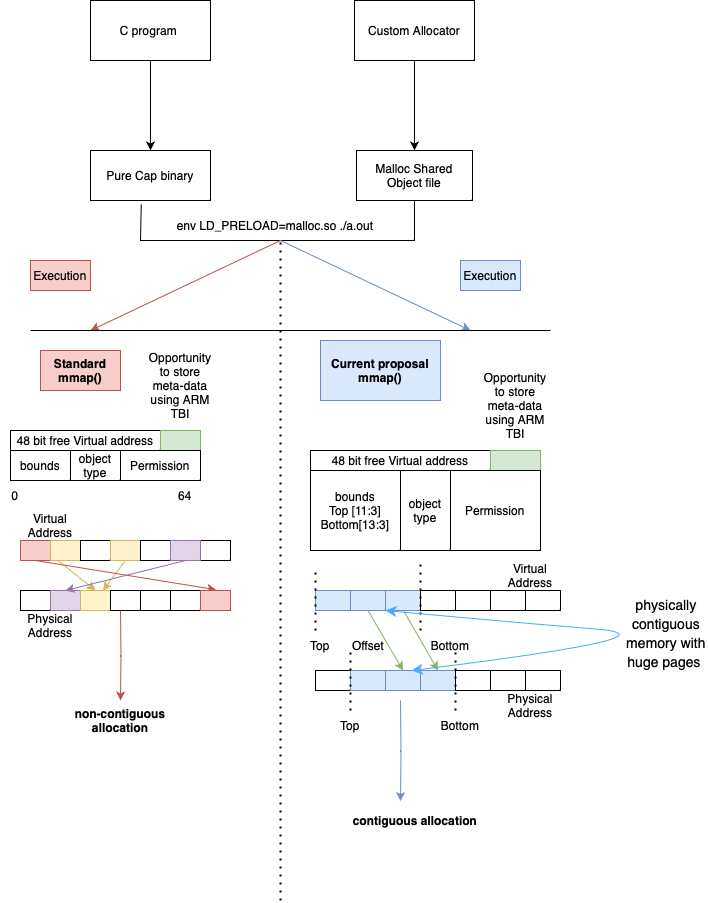
\includegraphics[width=0.6\textwidth]{diagrams/HighOverviewArchitecture24.png}
  \caption{High overview architecture}
  \label{fig:HighOverviewArchitecture}
% \end{minipage}
\end{figure}

% The figure above demonstrates the approach taken for using CHERI 
% 128bit FAT pointer scheme to allow a blocked based behavior on 
% on physically contiguous memory which is on the right against the 
% regular mmap approach which further elaborated in section (). The 
% green highlighted refers to the excess space available between 
% the 48th and 64th bit which can be used to store more meta-data which 
% is elaborated in the future work section().


Figure \ref{fig:HighOverviewArchitecture} illustrates the methodology employed to leverage the CHERI 
128-bit FAT-pointer scheme for facilitating block-based memory management
 on physically contiguous memory, which is depicted on the right side of the figure. 
 This technique contrasts with the conventional mmap approach.

In figure \ref{fig:HighOverviewArchitecture}, the green-highlighted section marks the unused space between the 48th and 64th bits
within the FAT-pointer. This area of unused bits presents an opportunity to store additional metadata,
potentially enhancing the capabilities of the memory management system. 
Here we explore how this additional metadata storage could be used to further optimize memory allocation.

% By employing the CHERI 128-bit FAT-pointer scheme, the approach depicted aims to streamline the management of memory blocks, ensuring they are physically contiguous. This is in contrast to the traditional mmap approach, which typically does not guarantee physical contiguity of allocated memory regions.


\section{Range creation and huge pages}
% \begin{minipage}[t]{0.4\linewidth}
\begin{figure}[h]
  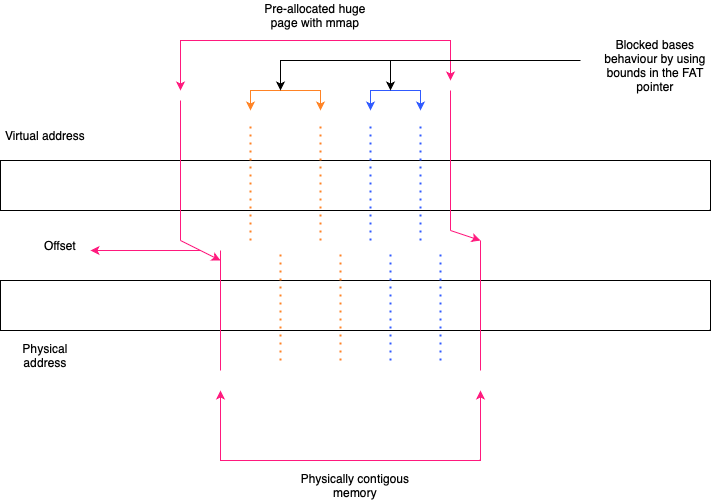
\includegraphics[width=0.8\textwidth]{diagrams/AllocationOverview24.png}
  \caption{Range of memory}
  \label{fig:RangeOfMemory}
\end{figure}
% \end{minipage}

% Ranges of memory are created based on bounds encoded to the FAT-Pointer based on the CHERI 128 bit 
% bounds compressed scheme. The Chuck between the specified upper and lower bounds are always physically
% contiguous. In the following implementation an arbitrary size huge page is initially allocated and within 
% this huge page custom size memory is allocated using a custom written mmap function which overwrites the existing block 
% based mmap function. Once memory is physically allocated using the custom mmap function call then bounds are set to it for tracking 
% the block of memory instead of using the TLB. 

In this implementation, memory ranges are established using bounds encoded within the FAT-pointer, adhering 
to the CHERI 128-bit bounds compression scheme\cite{woodruff_cheri_2019}. The memory chunk defined by the upper and lower bounds is 
always physically contiguous. Initially, a huge page of arbitrary size is allocated. Within this huge page, 
custom-sized memory segments are allocated using a custom-designed mmap function, which overrides the existing 
block-based mmap function. Once the memory is physically allocated through this custom mmap function, bounds 
are set to track the memory block, eliminating the need for traditional TLB usage for this purpose. Traditional TLB usage 
involves maintaining numerous TLB entries, often supplemented by an L2 TLB and other hierarchical structures, 
to translate virtual addresses to physical addresses. This approach requires multiple entries to handle various 
memory segments, leading to increased overhead and complexity in address translation. Conversely, 
the current approach streamlines this process by using a single TLB entry to translate multiple
 addresses within a contiguous memory range. This reduces the number of required TLB entries, 
 simplifying the translation process and improving efficiency. By consolidating address translations 
 into a single TLB entry, this method minimizes the overhead associated with managing numerous TLB entries 
 and leverages the bounds encoded within the FAT-pointer for efficient memory tracking and access. 
 This approach allows for precise and efficient memory management within the allocated huge page. 


%  The figure mentioned above demonstrates a simple use-case were the dark pink line refers to a huge page and 
%  the orange and blue lines are 2 equivalent to 2 Malloc calls allocating memory in different regions which in turn
%  emulates a block based memory allocator within a huge page using the bounds encoded in the FAT-Pointer.
\smallskip\noindent
Figure \ref{fig:RangeOfMemory} illustrates a straightforward use-case in which the dark pink line represents a single, 
large contiguous memory area, or huge page. Within this huge page, the orange and blue lines indicate 
two separate memory allocations equivalent to invoking malloc twice to allocate memory in distinct regions. 
This scenario simulates a block-based memory allocator operating within the confines of the huge page. 
The allocations leverage the bounds encoded in the FAT-pointer, ensuring tracking and efficient 
management of the allocated memory regions. By using the FAT-pointer bounds, this method maintains the 
integrity and contiguity of the allocated blocks within the huge page.

% This is done via the FreeBSD kernel Contiguous memory allocator. 

% \subsection{Fragmentation}
% The problem with standard allocators which are physically contiguous
% is that fragmentation is eminent since 
% Fragmentation is handled by using bounds as a mechanism to allocate in a block-based manner.
% Bounds are used to seek through Physically contigous 
% \subsection{Allocation with huge pages}

\section{Software Stack}
\begin{figure}[h]
% \begin{minipage}[t]{0.4\linewidth}
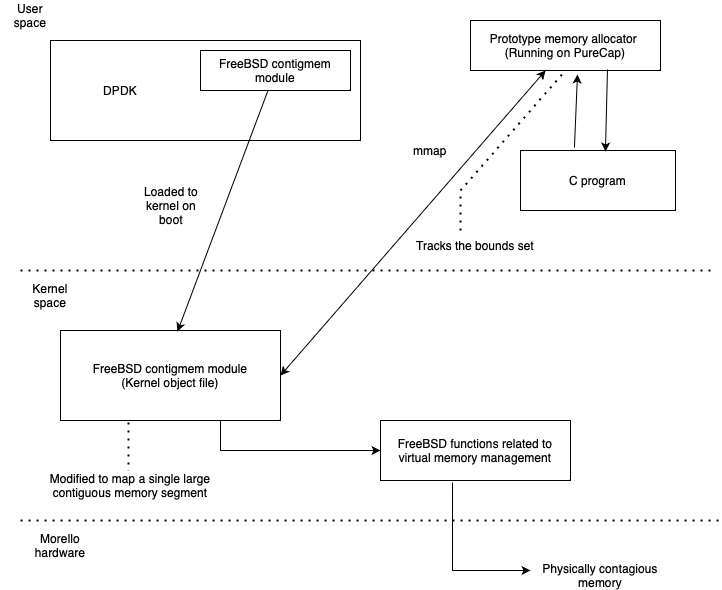
\includegraphics[width=0.8\textwidth]{diagrams/SoftwareStack24.png}
\caption{Overview of the software stack}
\label{fig:SoftwareStack}
% \end{minipage}
\end{figure}

% The Software stack consists of CHERIBSD as the base operating system due to official 
% support by ARM to the Morello's performance counters. As mentioned in the figure above 
% there is a C program that is linked to the prototype memory allocator or allocators benchmarked 
% against as mentioned in section (x) as either a Shared object file at compile time or as a header 
% file for smaller memory allocators. The modified mmap function call which is designed to be physically 
% contiguous is linked to the contigmem driver which is modified from the DPDK library (reference).
% The contigmem driver is loaded on boot time and reserves arbitrary size of a huge page which is
% set based on the experiment conducted. 

The software stack is based on CHERIBSD\cite{noauthor_getting_nodate}, selected because ARM officially supports Morello's performance 
counters\cite{noauthor_arm_nodate} on this operating system. As illustrated in the figure \ref{fig:SoftwareStack}, the setup includes a C program that 
is linked to the prototype memory allocator or to various memory allocators being benchmarked, as described 
in section~\ref{chap:evaluation}. This linkage can occur in two ways: either as a shared object file during compile time 
for larger allocators, or as a header file for smaller allocators, ensuring flexibility and efficiency 
in memory management.
\newline

This integration ensures that the memory allocation process is optimized for performance, leveraging the contiguity 
of memory blocks and the capabilities provided by the CHERI architecture and the Morello platform. By using the 
contigmem driver and the custom mmap function, the system achieves efficient memory allocation and tracking, 
crucial for the high-performance needs of the application.

\subsection{Contigmem driver from DPDK}
The custom mmap function, tailored to ensure physically contiguous memory allocation, is a key component 
of this system. This function is linked to the contigmem driver, which has been modified from the DPDK\cite{bi_dpdk-based_2016} library 
to meet the specific needs of this implementation. The contigmem driver is essential for managing large contiguous 
memory blocks and is loaded during the system boot process. It reserves a huge page of arbitrary size, with the 
size parameter set based on the requirements of the conducted experiments.

\begin{lstlisting}[language=C, caption=Contigmem driver , label=ContigInit]

MALLOC_DEFINE(M_CONTIGMEM, "contigmem", 
"contigmem(4) allocations");

static int contigmem_modevent(module_t mod, 
int type, void *arg)
{
	int error = 0;

	switch (type) {
	case MOD_LOAD:
		error = contigmem_load();
		break;
	case MOD_UNLOAD:
		error = contigmem_unload();
		break;
	default:
		break;
	}

	return error;
}

....

DECLARE_MODULE(contigmem, contigmem_mod, 
SI_SUB_DRIVERS, SI_ORDER_ANY);
MODULE_VERSION(contigmem, 1);

static struct cdevsw contigmem_ops = {
	.d_name         = "contigmem",
	.d_version      = D_VERSION,
	.d_flags        = D_TRACKCLOSE,
	.d_mmap_single  = contigmem_mmap_single,
	.d_open         = contigmem_open,
	.d_close        = contigmem_close,
};

static int
contigmem_load()
{
	....

	for (i = 0; i < contigmem_num_buffers; i++) {
		addr = contigmalloc(contigmem_buffer_size, 
           M_CONTIGMEM, M_ZERO,
		   0, BUS_SPACE_MAXADDR, 
           contigmem_buffer_size, 0);
	....
	}

    ....

error:
	for (i = 0; i < contigmem_num_buffers; i++) {
		if (contigmem_buffers[i].addr != NULL) {
			contigfree(contigmem_buffers[i].addr,
				contigmem_buffer_size, M_CONTIGMEM);
			contigmem_buffers[i].addr = NULL;
		}
		....
	}

	return error;
}

\end{lstlisting}

% The contigmem driver~\ref{ContigInit}  function is typically initialized during boot time but can be 
% loaded manually at any time using a Kernel load instruction. The cdevsw struct includes function pointers 
% that will be replaced when the driver is loaded. For example, the mmap function can be overwritten 
% when the driver is opened and used, as illustrated in the provided code snippets.

When the contigmem\_load~\ref{ContigInit} function is called, either during boot or when the Kernel module is loaded, it pre-allocates 
a segment of physically contiguous memory. This approach differs from FlexPointer\cite{chen_flexpointer_2023}, 
which allocates physically contiguous memory eagerly. The contigmem\_load function allocates memory using contigmalloc\cite{noauthor_contigmalloc9_nodate}, 
which allocates physically contiguous memory initialized to zero. The cdevsw struct refers to function 
calls which would be overwritten on loading the driver. In the code snippet~\ref{ContigInit} above
the mmap function would be overwritten with contigmem\_mmap\_single if the following driver is opened and truncated
as shown in Code snippet ~\ref{MallocSample}. 
\newline

In the code snippet ~\ref{ContigMmap} the cdev\_pager\_ops refers to the operations which will be overwritten 
when called with mmap such as overwriting page faults.

% Code snippet ~\ref{ContigInit} refers to the contigmem driver function when it 
% is initially which is normally loaded during boot time but can be loaded at any 
% point of time using Kernel load instruction. The cdevsw struct refers to function 
% calls which would be overwritten on loading the driver. In the code snippet above
% the mmap function would be overwritten if the following driver is opened and truncated
% as shown in Code snippet ~\ref{MallocInit}. The contigmem\_load function is called 
% when the Kernel module is loaded and it pre-allocates a segment of physically contigous
% memory unlike FlexPointer\cite{chen_flexpointer_2023} which eagerly allocates physically
% contigous memory. The contigmalloc function call allocates physically contigous Memory
% with the value 0. 

\begin{lstlisting}[language=C, caption=Contigmem driver mmap , label=ContigMmap]

static struct cdev_pager_ops contigmem_cdev_pager_ops = {
	.cdev_pg_ctor = contigmem_cdev_pager_ctor,
	.cdev_pg_dtor = contigmem_cdev_pager_dtor,
	.cdev_pg_fault = contigmem_cdev_pager_fault,
};

static int
contigmem_mmap_single(struct cdev *cdev, vm_ooffset_t 
*offset, vm_size_t size, struct vm_object **obj, int nprot)
{
    ....
	*obj = cdev_pager_allocate(vmh, OBJT_DEVICE, 
           &contigmem_cdev_pager_ops,size, nprot, 
           *offset, curthread->td_ucred);

	return 0;
}
\end{lstlisting}



\subsection{Sample memory allocator design}

\begin{lstlisting}[language=C, caption=Contigmem driver mmap , label=MallocSample]
   #define FILENAME "/dev/contigmem"
   void *ptr;
   int MallocCounter;

   size_t sizeUsed;
   
   ... 

   INITAlloc(void) {

   size_t sz;
   sz = 100000000;

   int fd = open(FILENAME, O_RDWR, 0600);

    if (fd < 0) {
        perror("open");
        exit(EXIT_FAILURE);
    }

    off_t offset = 0; // offset to seek to.

    if (ftruncate(fd, sz) < 0) {
        perror("ftruncate");
        close(fd);
        exit(EXIT_FAILURE);
    }

    ptr = mmap(NULL, sz,
    PROT_READ|PROT_WRITE, MAP_SHARED,fd,0);

   // Added error handling
    if(ptr == MAP_FAILED)
    {
        perror("mmap");
        exit(EXIT_FAILURE);
    }
    MallocCounter = (int)sz;
    }

    void* malloc(size_t sz)
    {
   sz = __builtin_align_up(sz, _Alignof(max_align_t));

   // printf("%d \n", sz);
   // printf("%d Malloc counter\n", MallocCounter);

   MallocCounter -= sz;
   void *ptrLink = &ptr[MallocCounter];
   ptrLink = cheri_setbounds(ptrLink, sz);

   return ptrLink;
     
   }

   void FREECHERI(void *ptr) { 

   // get length of free from bounds
   // in the pointer
   int len = cheri_getlen(ptr);

   munmap(ptr, len);
}

\end{lstlisting}

The code snippet~\ref{MallocSample} below shows a sample memory allocator
which is a really simple implementation that initially 
in the example allocates 1GB of memory using the mmap call which calls 
the mmap function from /dev/contigmem driver. This ensures memory allocated to the physically
contiguous memory allocated in the contigmem\_load() function using the contigmem\_mmap\_single()
function call in the kernel module, uses malloc 
and free to allocate within this memory chuck. The consideration of this is to ensure that a C program needs minor changes to use the benefit
using physically contiguous memory with bounds within a segment of memory.